\documentclass{beamer}\usepackage{graphicx, color}
%% maxwidth is the original width if it is less than linewidth
%% otherwise use linewidth (to make sure the graphics do not exceed the margin)
\makeatletter
\def\maxwidth{ %
  \ifdim\Gin@nat@width>\linewidth
    \linewidth
  \else
    \Gin@nat@width
  \fi
}
\makeatother

\IfFileExists{upquote.sty}{\usepackage{upquote}}{}
\definecolor{fgcolor}{rgb}{0.2, 0.2, 0.2}
\newcommand{\hlnumber}[1]{\textcolor[rgb]{0,0,0}{#1}}%
\newcommand{\hlfunctioncall}[1]{\textcolor[rgb]{0.501960784313725,0,0.329411764705882}{\textbf{#1}}}%
\newcommand{\hlstring}[1]{\textcolor[rgb]{0.6,0.6,1}{#1}}%
\newcommand{\hlkeyword}[1]{\textcolor[rgb]{0,0,0}{\textbf{#1}}}%
\newcommand{\hlargument}[1]{\textcolor[rgb]{0.690196078431373,0.250980392156863,0.0196078431372549}{#1}}%
\newcommand{\hlcomment}[1]{\textcolor[rgb]{0.180392156862745,0.6,0.341176470588235}{#1}}%
\newcommand{\hlroxygencomment}[1]{\textcolor[rgb]{0.43921568627451,0.47843137254902,0.701960784313725}{#1}}%
\newcommand{\hlformalargs}[1]{\textcolor[rgb]{0.690196078431373,0.250980392156863,0.0196078431372549}{#1}}%
\newcommand{\hleqformalargs}[1]{\textcolor[rgb]{0.690196078431373,0.250980392156863,0.0196078431372549}{#1}}%
\newcommand{\hlassignement}[1]{\textcolor[rgb]{0,0,0}{\textbf{#1}}}%
\newcommand{\hlpackage}[1]{\textcolor[rgb]{0.588235294117647,0.709803921568627,0.145098039215686}{#1}}%
\newcommand{\hlslot}[1]{\textit{#1}}%
\newcommand{\hlsymbol}[1]{\textcolor[rgb]{0,0,0}{#1}}%
\newcommand{\hlprompt}[1]{\textcolor[rgb]{0.2,0.2,0.2}{#1}}%

\usepackage{framed}
\makeatletter
\newenvironment{kframe}{%
 \def\at@end@of@kframe{}%
 \ifinner\ifhmode%
  \def\at@end@of@kframe{\end{minipage}}%
  \begin{minipage}{\columnwidth}%
 \fi\fi%
 \def\FrameCommand##1{\hskip\@totalleftmargin \hskip-\fboxsep
 \colorbox{shadecolor}{##1}\hskip-\fboxsep
     % There is no \\@totalrightmargin, so:
     \hskip-\linewidth \hskip-\@totalleftmargin \hskip\columnwidth}%
 \MakeFramed {\advance\hsize-\width
   \@totalleftmargin\z@ \linewidth\hsize
   \@setminipage}}%
 {\par\unskip\endMakeFramed%
 \at@end@of@kframe}
\makeatother

\definecolor{shadecolor}{rgb}{.97, .97, .97}
\definecolor{messagecolor}{rgb}{0, 0, 0}
\definecolor{warningcolor}{rgb}{1, 0, 1}
\definecolor{errorcolor}{rgb}{1, 0, 0}
\newenvironment{knitrout}{}{} % an empty environment to be redefined in TeX

\usepackage{alltt}
\usetheme{Stats}
\setbeamercovered{transparent}
\usepackage{color}
\usepackage{hyperref}
  \hypersetup{
  	colorlinks=true
		linkcolor=black
		}
\usepackage{url}
\usepackage{graphics}
\usepackage{tikz}
\usepackage{booktabs}





%%%%%%%%%%%%%%%%%%%%%%%%%%%%%%%% Title Slide %%%%%%%%%%%%%%%%%%%%%%%%%%
\title[]{Intro to Social Science Data Analysis \\[1cm] Week 11: Simple Linear Regression}
\author[]{
    \href{mailto:gandrud@yonsei.ac.kr}{Christopher Gandrud}
}
\date{\today}


\begin{document}

\frame{\titlepage}

\section[Outline]{}
\frame{\tableofcontents}

\section{Recap}
\frame{
	\frametitle{Quick Quiz 1}
  Find the sample proportions of the following party's supporters:
  \begin{table}
    \begin{tabular}{c c c c}
    \hline
    Saenuri & DUP & Other & Total \\
    \hline\hline
    1064 & 891 & 520 & 2475 \\ 
    \hline
    \end{tabular}
  \end{table}
}

\frame{
  \frametitle{Quick Quiz 1}
  \begin{table}
    \begin{tabular}{c c c c}
    \hline
    Saenuri & DUP & Other & Total \\
    \hline\hline
    1064 & 891 & 520 & 2475 \\ 
    (0.43) & (0.36) & (0.21) & (1) \\
    \hline
    \end{tabular}
  \end{table}
}

\frame{
  \frametitle{Quick Quiz 2}
  If we wanted to make inferences about {\bf{population proportions}} from sampling proportions, what {\bf{distribution}} do we often assume the sampling proportions follow? \\[0.5cm]
  
  What are it's {\bf{parameters}}?
}

\frame{
  \frametitle{Quick Quix 3}
  Imagine we have a two-way contingency table.
  \begin{table}
    \begin{tabular}{c c c c}
    \hline
     & Attend University & No University \\
    \hline\hline
    Married &&\\ 
    Not Married && \\
    \hline
    \end{tabular}
  \end{table}
  If we conducted a $\chi^{2}$ test with this data and found a p-value of $<0.001$ what would we conclude?
}

\frame{
  \frametitle{Quick Quiz 4}
  Write the simple linear regression equation for how a person's height is related to their income.
}

\frame{
  \frametitle{Quick Quiz 5}
  Describe how a linear regression line would look if the relationship between two variables was negative. \\[0.5cm]
  How would it look if the relationship was positive? \\[0.5cm]
  What about no relationship?
}

%%%%%%%%%%%% Correlation
\section{Correlation}
\frame{
  \framtitle{Motivation}
  Since almost no interesting relationship is perfectly linear, how do we find the {\bf{best fit line}} that describes the relationship between some $x$ and some $y$?
}

\frame{
  \frametitle{How?}
  \begin{center}
    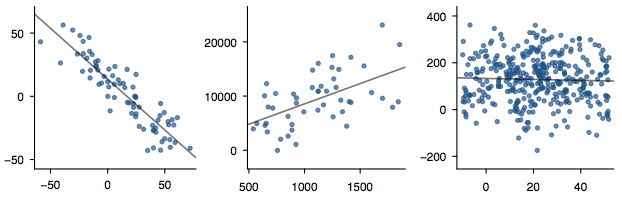
\includegraphics[scale=0.5]{/git_repositories/Introduction_to_Statistics_and_Data_Analysis_Yonsei/Lectures/Lecture10/ExampleSLR.png} \\[0.5cm]
  \end{center}  
{\tiny{Source: Diaz et. al. (2011, 216)}}
}

\frame{
  In {\bf{simple linear regression}} we are trying to find the straight line that is {\bf{as close to all of the data points as possible}}.\\[1cm]
  How do we find this line?
}

\frame{
  \frametitle{How?}
  \begin{center}
    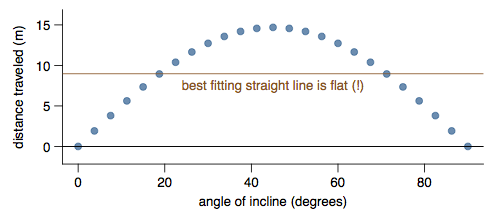
\includegraphics[scale=0.5]{/git_repositories/Introduction_to_Statistics_and_Data_Analysis_Yonsei/Lectures/Lecture10/NonLinear.png} \\[0.5cm]
  \end{center}  
{\tiny{Source: Diaz et. al. (2011, 216)}}
}

\begin{frame}[fragile]
  Let's use the SAT/GPA data from the \texttt{openintro} package:
\begin{knitrout}
\definecolor{shadecolor}{rgb}{0.969, 0.969, 0.969}\color{fgcolor}\begin{kframe}
\begin{alltt}
\hlcomment{# Load library}
\hlfunctioncall{library}(openintro)

\hlcomment{# Load data}
\hlfunctioncall{data}(satGPA)

\hlcomment{# Show variables}
\hlfunctioncall{names}(satGPA)
\end{alltt}
\begin{verbatim}
## [1] "sex"    "SATV"   "SATM"   "SATSum" "HSGPA" 
## [6] "FYGPA"
\end{verbatim}
\begin{alltt}

\hlcomment{# Subset to remove the sex variable}
satGPASlim <- satGPA[, 2:6]
\end{alltt}
\end{kframe}
\end{knitrout}

\end{frame}

\begin{frame}[fragile]
  \frametitle{Plot the SAT Scores \& GPAs}
\begin{knitrout}
\definecolor{shadecolor}{rgb}{0.969, 0.969, 0.969}\color{fgcolor}\begin{kframe}
\begin{alltt}
\hlfunctioncall{library}(GGally)

\hlfunctioncall{ggpairs}(satGPASlim, upper = \hlstring{"blank"})
\end{alltt}
\end{kframe}

{\centering 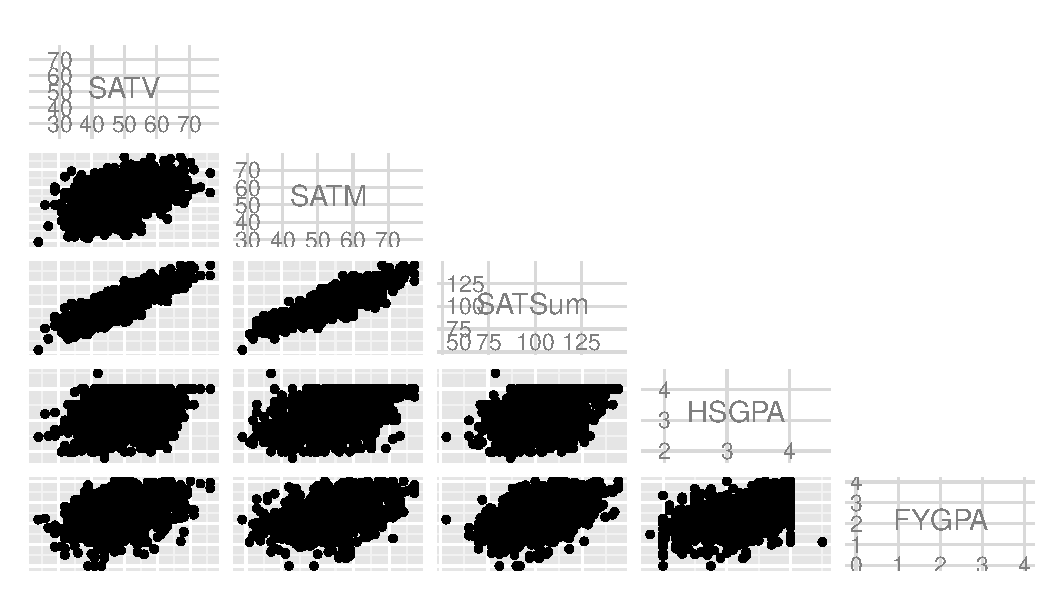
\includegraphics[width=\maxwidth]{figure/DescribeGPA} 

}


\end{knitrout}

\end{frame}

\begin{frame}[fragile]
  \frametitle{First Year GPA}
  Universities want to know how well student's total SAT scores (\texttt{SATSum}) relate to their academic performance in the first year of university (\texttt{FYGPA}.
\begin{knitrout}
\definecolor{shadecolor}{rgb}{0.969, 0.969, 0.969}\color{fgcolor}

{\centering 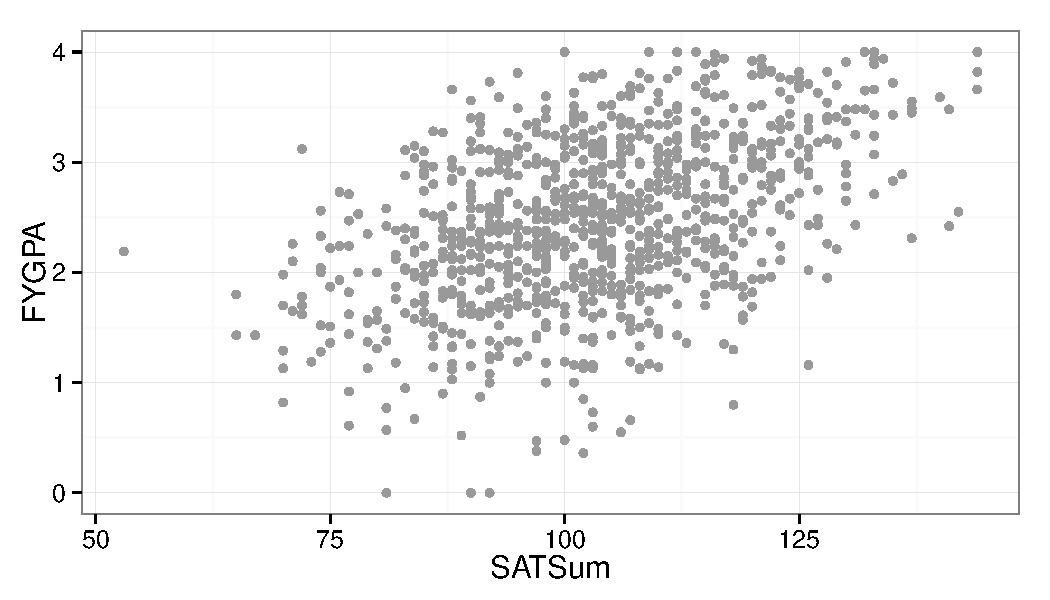
\includegraphics[width=\maxwidth]{figure/SATFYGPA} 

}


\end{knitrout}

\end{frame}

\frame{
  \frametitle{Correlation}
  One way to describe the overall relationship between \texttt{SATSum} and \texttt{FYGPA} is to find the {\bf{correlation}} between the two variables. 
}

\frame{
  \frametitle{Correlation}
{\LARGE{Correlation ($R$):}} \\[0.5cm]
  Describes the {\bf{strength}} of a linear relationship. \\[0.25cm]
  It ranges from -1 to 1. \\[0.5cm]
  -1 indicates a {\bf{perfect negative relationship}}.\\[0.25cm]
  1 indicates a {\bf{perfect positive relationship}}. \\[0.25cm]
  0 indicates {\bf{no correlation/relationship}}.  
}

\frame{
  \frametitle{Correlation}
  To find the correlation for observations $(x_{1}, y_{1}),\:(x_{2}, y_{2})\ldots(x_{n}, y_{n})$
\[
  R = \frac{1}{n - 1}\sum\limits_{i = 1}^n\frac{x_{i} - \bar{x}}{s_{x}}\frac{y_{i} - \bar{y}}{s_{y}}
\] 
}

\begin{frame}[fragile]
  \frametitle{Or\ldots}
  Or we can have R do the maths for us.
\begin{knitrout}
\definecolor{shadecolor}{rgb}{0.969, 0.969, 0.969}\color{fgcolor}\begin{kframe}
\begin{alltt}
\hlfunctioncall{cor}(satGPA$SATSum, satGPA$FYGPA)
\end{alltt}
\begin{verbatim}
## [1] 0.4603
\end{verbatim}
\end{kframe}
\end{knitrout}

\end{frame}

\frame{
  \frametitle{Statistical Significance \& Correlation}
  If we wanted to test to see if the correlation is statistically significant, what would the null hypothesis be?
}

\frame{
  \frametitle{Statistical Significance \& Correlation}
{\large{$H_{0}$: $R = 0$ \\[0.5cm]
$H_{a}$: R \neq 0$}} 
}

\begin{frame}[fragile]
  \frametitle{Hypothesis Testing Correlation Coefficients in R}
\begin{knitrout}
\definecolor{shadecolor}{rgb}{0.969, 0.969, 0.969}\color{fgcolor}\begin{kframe}
\begin{alltt}
\hlfunctioncall{cor.test}(satGPA$SATSum, satGPA$FYGPA)
\end{alltt}
\begin{verbatim}
## 
## 	Pearson's product-moment correlation
## 
## data:  satGPA$SATSum and satGPA$FYGPA 
## t = 16.38, df = 998, p-value < 2.2e-16
## alternative hypothesis: true correlation is not equal to 0 
## 95 percent confidence interval:
##  0.4100 0.5078 
## sample estimates:
##    cor 
## 0.4603
\end{verbatim}
\end{kframe}
\end{knitrout}

\end{frame}

\frame{
  \frametitle{More Correlation Examples}
  \begin{center}
  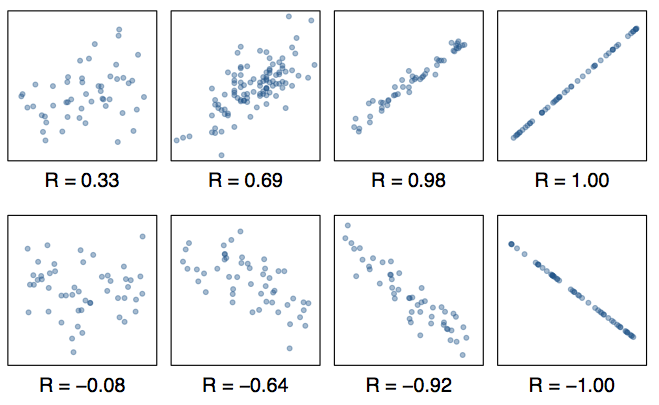
\includegraphics[scale=0.45]{LinearCor.png} \\[0.5cm]
  \end{center}
{\tiny{Source: Diaz et al. (2011, 282 )}}
}

\frame{
  \frametitle{Caution}
  A low linear correlation {\bf{does not necessarily}} mean a weak relationship. \\[0.5cm]
  It means a weak {\bf{linear}} relationship.
  \begin{center}
  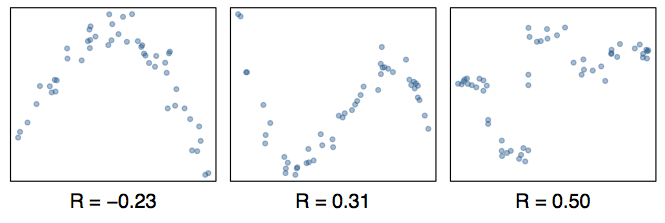
\includegraphics[scale=0.45]{NonLinearCor.png} \\[0.5cm]
  \end{center}
{\tiny{Source: Diaz et al. (2011, 282 )}}
}

%%%%%%%%%%%% Least Squares Regression
\section{Best Fit Lines \& Least Squares Regression}
\frame{
  \frametitle{Best Fit Lines \& Least Squares Regression}
  Ok, linear correlations are useful for finding:
  \begin{itemize}
    \item the {\bf{direction}} of a linear relationship,
    \item the {\bf{strength}} of a linear relationship.
  \end{itemize}
}

\frame{
  \frametitle{More specific}
  What if we want to be more specific? \\[0.5cm]
  For example, using a student's total SAT score to predict their first year university GPA.\\[0.5cm]
{\bf{Note:}} the estimated value of the dependent variable ($y$) is often written $\hat{y}$ ({\emph{``y hat"}}).

}

\begin{frame}[fragile]
  \frametitle{The Linear Best Fit Line}
  The blue line is the closest straight line (``best fit") to all of the data points.
\begin{knitrout}
\definecolor{shadecolor}{rgb}{0.969, 0.969, 0.969}\color{fgcolor}

{\centering 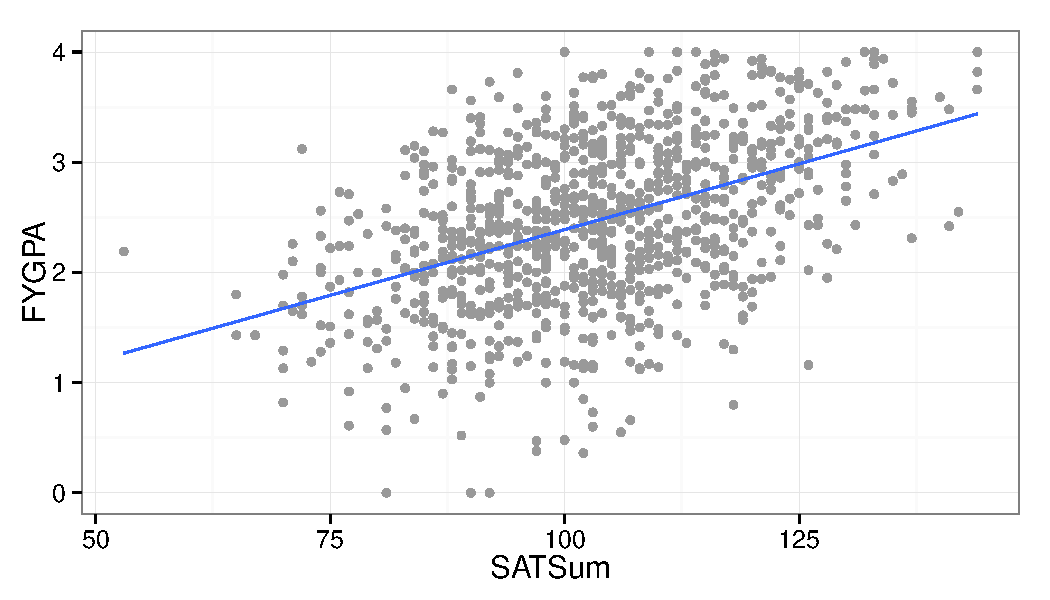
\includegraphics[width=\maxwidth]{figure/BestFit} 

}


\end{knitrout}

\end{frame}

\frame{
  \frametitle{How?}
  \begin{center}
    {\LARGE{How do we find the best fit line?}}
  \end{center}
}

\frame{
  \frametitle{Residuals}
  Well, the best fit line would do something like have the smallest {\bf{residuals}} possible. \\[0.5cm]
  What is a residual?
}

\frame{
  \frametitle{Residuals}
{\LARGE{Residual:}} \\[0.5cm]
  the difference between the observed and expected values based on the best fit model.\\[0.5cm]
  More formally: the residual ($e_{i}$) of the observation $(x_{i}, y_{i})$ is the difference between the observed value of $y_{i}$ and the expected value $\hat{y}_{i}$:
  \[
  e_{i} = y_{i} - \hat{y}_{i}
  \]
}

\begin{frame}[fragile]
  \frametitle{Residuals}
  The red point is at (81, 0.77). Given that \texttt{SATSum} is 81, it is expected to be at 1.935. So, it's residual is $0.77 - 1.935 = -1.65$.
\begin{knitrout}
\definecolor{shadecolor}{rgb}{0.969, 0.969, 0.969}\color{fgcolor}

{\centering 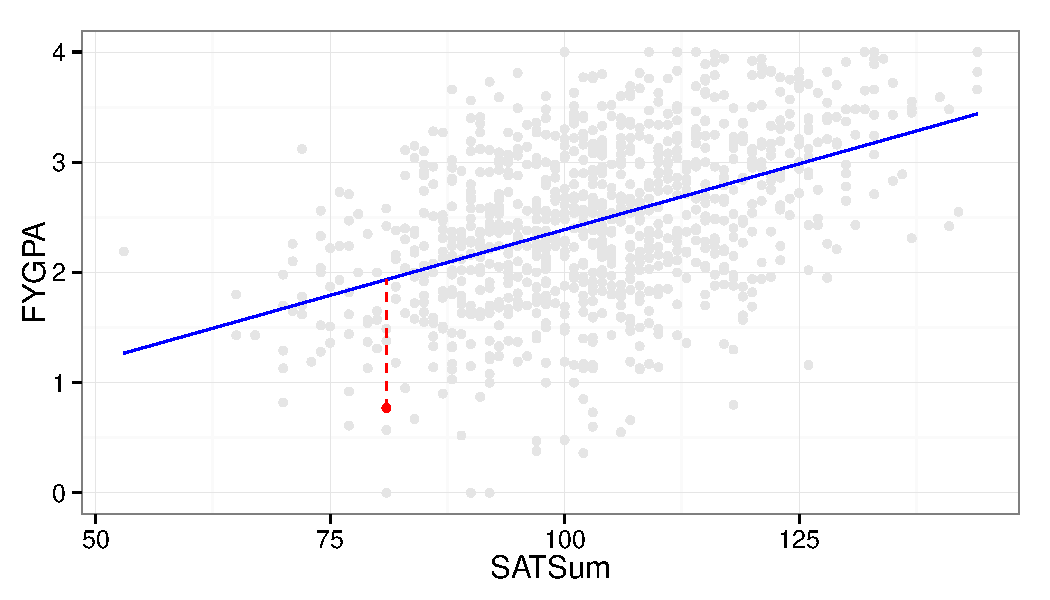
\includegraphics[width=\maxwidth]{figure/Res1} 

}


\end{knitrout}

\end{frame}

\begin{frame}[fragile]
  \frametitle{Residuals}
  The red point is at (124, 3.44). Given that \texttt{SATSum} is 124, it is expected to be at 2.94. So, it's residual is $3.44 - 2.94 = 0.5$.
\begin{knitrout}
\definecolor{shadecolor}{rgb}{0.969, 0.969, 0.969}\color{fgcolor}

{\centering 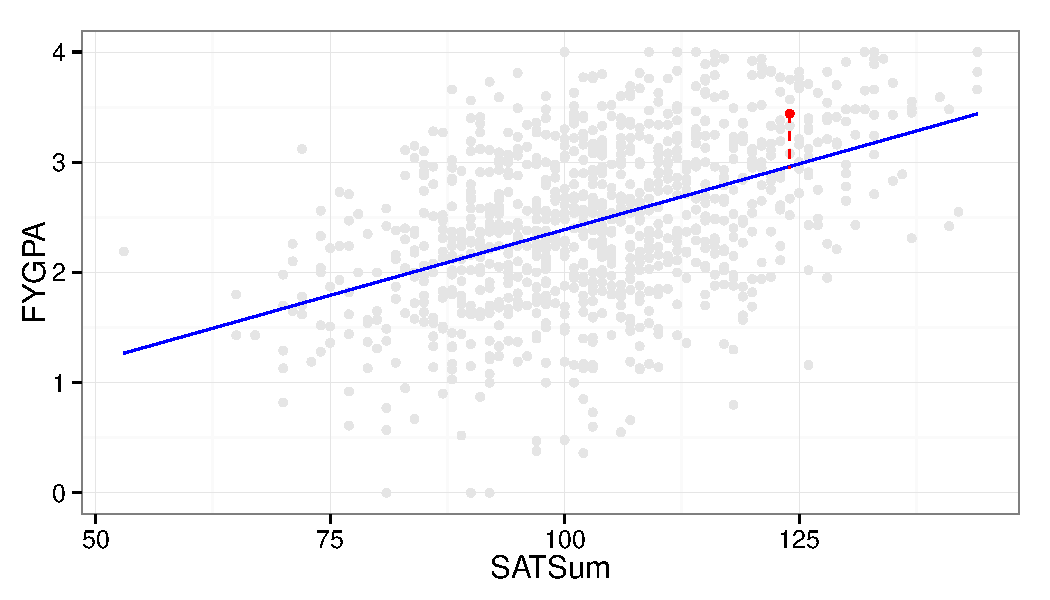
\includegraphics[width=\maxwidth]{figure/Res2} 

}


\end{knitrout}

\end{frame}

%%%%%%%%% Special Issues
\section{Some Special Issues in Simple Linear Regression}
\frame{
  \frametitle{Outliers}
}

\frame{
  \frametitle{Dummy Variables}
  So far we have only looked at creating simple linear regression models with {\bf{continuous numeric}} dependent and independent variables. \\[0.5cm]
  What if we have a continuous dependent variable and a dichotomous independent variable?
}

\frame{
  \frametitle{Categorical Dependent}
  What if our {\bf{dependent variable}} is categorical, for example, the party someone voted for? \\[0.5cm]
  For these situations you need to use a different type of regression, usually {\bf{logistic regression}}. \\[0.5cm]
  We do not cover this type of regression in this course.
}

\frame{
  \frametitle{Caution: Non-Linear Relationships}
  It is always a good idea to check for {\bf{non-linear relationships}}.
}

\frame{
  One way to address non-linear relationships is to {\bf{transform}} the data using, for example: \\[0.5cm]
  \begin{itemize}
    \item logs
    \item squares, cubes.
  \end{itemize}
}





\begin{frame}[allowframebreaks]
  \frametitle{References}
  Crawley, Michael J. 2005. Statistics: An Introduction Using R. Chichester: John Wiley & Sons. Ltd. \\[0.25cm]
  Diaz, David M., Christopher D. Barr, and Mine \c{C}etinkaya-Rundel. 2011. OpenIntro Statistics. 1st ed. \url{http://www.openintro.org/stat/downloads.php}. \\[0.25cm] 
\end{frame}


\end{document}
